\documentclass{article} 
\usepackage{amsmath} 
\usepackage{amssymb} 
\usepackage{amsthm} 
\usepackage[margin=0.2in]{geometry} 
\usepackage{hyperref} 
\usepackage{physics} 
\usepackage{tikz} 
\usepackage{mathtools}
\usepackage{graphicx}\graphicspath{{./images/}}
\mathtoolsset{showonlyrefs} 
\theoremstyle{definition} 
\newtheorem{theorem}{Theorem}[section] 
\newtheorem{corollary}{Corollary}[theorem] 
\newtheorem{lemma}[theorem]{Lemma} 
\newtheorem{definition}{Definition}[section] 

\author{Connor Duncan}
\date{\today}

\title{notes-11-15-2019}
\begin{document}
\abstract{A single document copy of these notes, as well as a mirror of every note, can be found at \url{connorduncan.xyz/notes}}
\subsection{Fermi's Golden Rule: Redux} FGR is a simple formula that we really don't need to rederive. \begin{equation}\label{eq:fgr} W_i(\omega)=\frac{2\pi}{\hbar}\left(\left|V_i(\omega)\right|^2\rho(E_i+\hbar\omega)+|V_i(-\omega)|^2\rho(E_i-\omega)\right) \end{equation} where \begin{equation} |V_i(\omega)|^2=|\bra{f}V\ket{i}|^2 \end{equation} which we have to evaluate with resolution of identity to get \begin{equation} \int_{}^{}dxdx'\bra{f}\ket{x}\bra{x}V\ket{x'}\bra{x'}\ket{i} \end{equation} Also, in the fourth problem on the last set, where we have \begin{equation} V(t)=V\cos(\omega t)\mathbb{I}\otimes\sigma^x \end{equation} which acts on the wavefunction $\ket{\psi}\otimes\ket{\sigma}$. This is going to make our function \begin{equation} \bra{\psi_f}\mathbb{I}\otimes\sigma^x\ket{\psi_i}=\int_{}^{}d^3x\varphi_{f\uparrow}^*\varphi_{i\downarrow} \end{equation} which, we can use plane waves as the basis \begin{equation} \psi_{\downarrow}=\frac{1}{(2\pi x_0)^{1/4}}e^{r^2/4x_0^2} \end{equation} and \begin{equation} \psi_\uparrow=\frac{1}{\sqrt{V}}e^{-i\vec{k}\cdot\vec{x}} \end{equation} This is going to fall off as an exponential, after some initial rise. It'll be a peaked function. \subsection{Nearly Resonant Perturbation} We'll consider the following \begin{center} \begin{tikzpicture} \node (e) at (2,1) {$\ket{e}$}; \node (g) at (2,-1) {$\ket{g}$}; \draw (0,1) -- (e); \draw (0,-1) -- (g); \draw[<->] (-0.2,-1) -- (-0.2,1.2) node[anchor=east] {$\hbar\omega$}; \draw[<->] (-0.1,1)--(-0.1,1.2) node[anchor=west] {$\hbar\Delta\omega$}; \end{tikzpicture} \end{center} We're going to end up with \begin{align} P_{ge}^{(1)}(t)=\frac{2}{\hbar^2}|A^\dag_{ge}|^2F(t,\Delta\omega)t \\ =\frac{4|A_{ge}^\dag|^2}{(\hbar\Delta\omega)^2}\sin^2(\Delta\omega t/2) \end{align} and where $\Delta\omega\rightarrow 0$ we should have some divergence where this goes to \begin{equation} \frac{1}{\hbar^2}|A_{eg}|^2t^2 \end{equation} which can be larger than one. This is bad. So, we need to step back and rewrite the hamiltonain, solving the schroedinger equation \begin{equation} H=H_0+H_1(t) \end{equation} where \begin{equation} G_1(t)=\left(\hat Ae^{-i\omega t}+\hat A^\dag e^{i\omega t}\right)\mathcal{V}(t) \end{equation} We take our usual \begin{equation} d_n(t)=e^{-iE_nt}c_n(t) \end{equation} so the schroedinger equaiton has to become \begin{equation} i\hbar\dot{d}_m=\sum_{n}^{}\left[A_{mn}e^{-i(\omega_{mn}-\omega)t}+A^\dag_{mn}e^{-i(\omega_{mn}+\omega)t}\right]d_n(t) \end{equation} If we think about the exactly resonant term, our first exponent becomes non-oscillating. On strongly oscillating terms. on reaosnable time scales this is going to average out to becomes zero. So we can ignore non-resonant terms, but we need to leave terms which don't oscillate. So, our schroedinger equation now becomes in terms of \begin{align} i\hbar\dot d_e=A_{ge}e^{i\Delta\omega t}d_g && \downarrow=e \\ i\hbar\dot d_g=A_{ge}^\dag e^{-i\Delta\omega t}d_e && \uparrow=g \end{align} So, we have \begin{equation} i\hbar\begin{bmatrix}\dot d_g\\\dot d_e\end{bmatrix} = \begin{bmatrix} 0 & -\frac{B}{2}e^{-i\varphi}e^{-i\Delta\omega t}\\ -\frac{B}{2}e^{i\varphi} e^{i\Delta\omega t} & 0 \end{bmatrix} \begin{bmatrix}d_g\\d_e\end{bmatrix} \end{equation} we can think about making this into a spin-${1\over 2}$ system \begin{equation} i\hbar\ket{\chi}=\hat H\ket{\chi} \end{equation} where \begin{equation} \hat H=-\frac{B}{2}\cos(\Delta\omega t+\varphi)\sigma^x-\frac{B}{2}\sin(\Delta\omega t+\varphi)\sigma^y \end{equation} This looks like a spin-1/2 rotating magnetic field \subsubsection{Exact Resonance $\Delta\omega=0$ (Rabi Oscillations)} We now have a perfect spin${1\over2}$ system in a static field \begin{equation} H=-\frac{1}{2}\vec{B}\cdot\vec{\sigma} \end{equation} which gives \begin{equation} \ket{\psi(t)}e^{-iHt}\ket{\psi(0)}=e^{-\frac{i}{2}B\cdot\sigma t}\ket{\uparrow} \end{equation} So, the rotation goes as $\theta=Bt$, with frequency $\Omega=B$. If we pick $\varphi=0$, then we have \begin{equation} \ket{\psi(t)}=\cos(\frac{1}{2}\Omega t)\ket{\uparrow}-i\sin(\frac{1}{2}\Omega t)\ket{\downarrow} \end{equation} with \begin{equation} P_e(t)=\sin[2](\frac{\Omega}{2}t) \end{equation} which gives \begin{center} 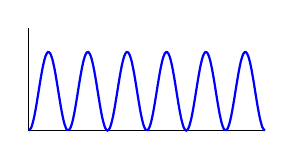
\begin{tikzpicture} \draw (0,0)--(0,1.3); \draw (0,0)--(3,0); \draw[blue,thick] plot[domain=0:3,variable=\x,smooth,samples=100] ({\x},{sin(\x*360)^2}); \end{tikzpicture} \end{center} \subsubsection{Off Resonant Case} We're going to pick an axis to remain in the direction of the field, and change the basis with a unitary operator which eliminates the rotation of the field. IIRC we did this in 137A? We're going to pick some unitary transformation so that we are in the rotating frame of reference. We can let $R(t)=e^{-\frac{i}{2}\Delta\omega t\sigma^z}$, so we get \begin{align} \ket{\tilde\uparrow}=R(t)\ket{\uparrow}=e^{-\frac{i}{2}\Delta\omega t}\ket{\uparrow} && \ket{\tilde\downarrow}=R(t)\ket{\downarrow}=e^{\frac{i}{2}\Delta\omega t}\ket{\downarrow} \end{align} which gives \begin{align} \ket{\psi(t)}=d_\uparrow(t)\ket{\uparrow}+d_\downarrow(t)\ket{\downarrow} \\ =d_\uparrow(t)e^{\frac{i}{2}\Delta\omega t}\ket{\tilde\uparrow}+d_\downarrow(t)e^{-\frac{i}{2}\Delta\omega t}\ket{\tilde\downarrow} \end{align} Our new schroedinger equation becomes \begin{align} i\hbar\pdv{t}d_{\updownarrow}(t)=i\hbar\pdv{t}\left[e^{\mp\frac{i}{2}\Delta\omega t}\tilde d_\updownarrow(t)\right] =i\hbar\left[ \mp\frac{i}{2}\Delta\omega e^{\mp\frac{i}{2}\Delta\omega t}\tilde d_\updownarrow(t)+ e^{\mp\frac{i}{2}\Delta\omega t}\dot{\tilde d}_\updownarrow(t) \right] \end{align} This ends up coming out as \begin{equation} i\hbar\pdv{t}d_{\uparrow,\downarrow}(t)=-\frac{B}{2}e^{\mp i\Delta\omega t}d_{\downarrow,\uparrow}=-\frac{B}{2}\tilde d_{\downarrow,\uparrow}(t) \end{equation} more or less. We super ran out of time. Basically, we can get a time independent effective hamiltonian in our new basis, and rotate back to the old basis to get the result.
\end{document}
